\documentclass[conference]{IEEEtran}
%\IEEEoverridecommandlockouts
% The preceding line is only needed to identify funding in the first footnote. If that is unneeded, please comment it out.
\usepackage{cite}
\usepackage{amsmath,amssymb,amsfonts}
\usepackage{algorithmic}
\usepackage{graphicx}
\usepackage{textcomp}
\usepackage{xcolor}
\usepackage{cuted}
\usepackage{tikz}
\usepackage{pgfplots}
\usepackage{url}


\usetikzlibrary{calc,trees,positioning,arrows,chains,shapes.geometric,%
    decorations.pathreplacing,decorations.pathmorphing,shapes,%
    matrix,shapes.symbols}

\tikzstyle{line} = [draw, -, thick]
\tikzstyle{nodraw} = [draw, fill, circle, minimum width=0pt, inner sep=0pt]
\tikzstyle{box} = [line, rectangle, rounded corners, text centered]

\tikzset{
>=stealth',
  punktchain/.style={
    rectangle, 
    rounded corners, 
    draw=black, very thick,
    text width=2em, 
    minimum height=3em, 
    text centered, 
    on chain},
  line/.style={draw, thick, <-},
  element/.style={
    tape,
    top color=white,
    bottom color=blue!50!black!60!,
    minimum width=1em,
    draw=blue!40!black!90, very thick,
    text width=2em, 
    minimum height=3.5em, 
    text centered, 
    on chain},
  every join/.style={->, thick,shorten >=1pt},
  decoration={brace},
  tuborg/.style={decorate},
  tubnode/.style={midway, right=2pt},
}


\def\BibTeX{{\rm B\kern-.05em{\sc i\kern-.025em b}\kern-.08em
    T\kern-.1667em\lower.7ex\hbox{E}\kern-.125emX}}
\newcommand*\Laplace{\mathop{}\!\mathbin\bigtriangleup}
\begin{document}

\title{Combining checkpointing and data compression\\ for large scale seismic inversion}

\author{\IEEEauthorblockN{Navjot Kukreja}
\IEEEauthorblockA{%\textit{Department of Earth Science and Engineering} \\
\textit{Imperial College London}\\
London, UK \\
n.kukreja@imperial.ac.uk}
\and
\IEEEauthorblockN{Jan H\"uckelheim}
\IEEEauthorblockA{%\textit{Department of Earth Science and Engineering}\\
\textit{Imperial College London}\\
London, UK }
\and
\IEEEauthorblockN{Mathias Louboutin}
\IEEEauthorblockA{%\textit{School of Computational Science and Engineering} \\
\textit{Georgia Institute of Technology}\\
Atlanta, GA, USA\\}
\and
\IEEEauthorblockN{Kaiyuan Hou}
\IEEEauthorblockA{%\textit{Department of Electrical Engineering and Computer Science} \\
\textit{Northwestern University}\\
Evanston, IL, USA \\
}
\and
\IEEEauthorblockN{Fabio Luporini}
\IEEEauthorblockA{%\textit{Department of Earth Science and Engineering} \\
\textit{Imperial College London}\\
London, UK \\
}
\and
\IEEEauthorblockN{Paul Hovland}
\IEEEauthorblockA{%\textit{Mathematics and Computer Science Division} \\
\textit{Argonne National Laboratory}\\
Lemont, IL, USA \\
}
\and
\IEEEauthorblockN{Gerard Gorman}
\IEEEauthorblockA{%\textit{Department of Earth Science and Engineering}\\
\textit{Imperial College London}\\
London, UK }
}

\maketitle

\begin{abstract}
Seismic inversion and imaging are adjoint-based optimization problems that processes up to terabytes of data, regularly exceeding the memory
capacity of available computers. Data compression is an effective strategy to
reduce this memory requirement by a certain factor, particularly if some loss in
accuracy is acceptable. A popular alternative is checkpointing, where data is
stored at selected points in time, and values at other times are recomputed as
needed from the last stored state.  This allows arbitrarily large adjoint
computations with limited memory, at the cost of additional recomputations.

In this paper we combine compression and checkpointing for the first
time to compute a realistic seismic inversion. The combination of
checkpointing and compression allows
larger adjoint computations compared to using only compression, and
reduces the recomputation overhead significantly compared to using only checkpointing.
\end{abstract}

\begin{IEEEkeywords}
Checkpointing, compression, adjoints, inversion
\end{IEEEkeywords}

\section{Introduction}
Adjoint-based optimization problems typically consist of a simulation that is
run forward in simulation time, producing data that is used in reverse order by
a subsequent adjoint computation that is run backwards in simulation time.
Figure~\ref{fig:dataflow} shows the resulting data flow. Many important
applications in science and engineering have this structure, including
seismic inversion.

In seismic inversion, the propagation of seismic waves through the earth's subsurface is simulated and compared with data from field measurements. The model of the subsurface is iteratively improved by minimizing the misfit between simulated data and field measurement in an adjoint optimization problem.
Figure~\ref{fig:offshore_survey} shows the setup of the field experiment that produces the measured data~\cite{plessix2006review}. Storing all intermediate
results as required for the data flow shown in Figure~\ref{fig:dataflow} is not
feasible, since this would require tens of terabytes of memory, which is not
commonly available on the machines used to solve these problems. To solve this
problem, a number of strategies are used that are discussed in the following
paragraphs. While this paper uses seismic inversion as a test case, most of these ideas, including the one presented in this work, are also applicable to other adjoint optimization problems.

\begin{figure}
\begin{center}
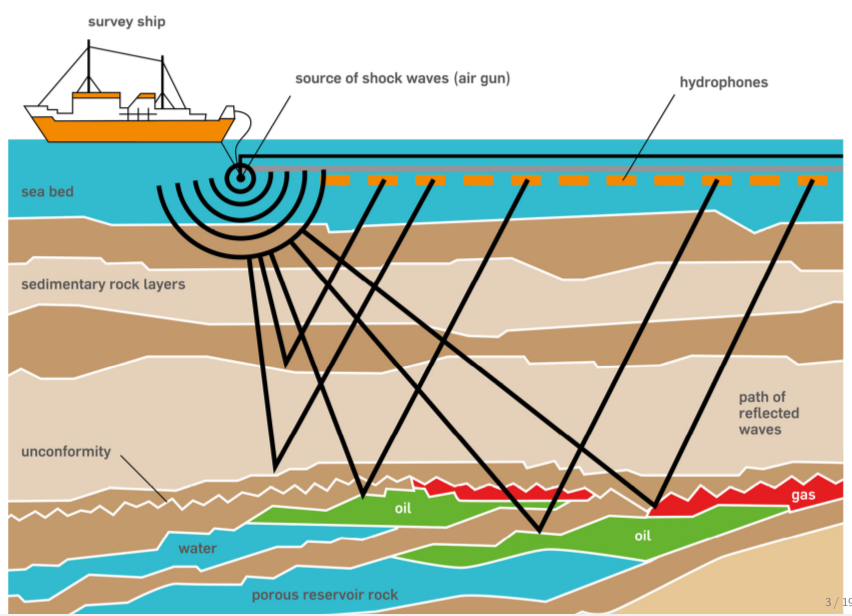
\includegraphics[width=0.8\linewidth]{images/survey-ship-diagram.png}
\end{center}
\caption{Illustration of an offshore seismic survey that collects the input data for seismic inversion}
\label{fig:offshore_survey}
\end{figure}

Domain decomposition is often used not only to distribute the computational
workload across more processors, but also to utilize the large amount of memory
available in distributed systems. While this strategy is very powerful, the
number of compute nodes and therefore the amount of memory that can be used
efficiently is limited, for example by communication overheads that start to
dominate as the domain is split into increasingly small pieces~\cite{virieux2009seismic}. Secondly, this method is broadly used on conventional clusters but can be drastically more complicated to seup and slower due to the communication in the Cloud.
Another common strategy in seismic inversion is to only store values at the boundaries of the domain at each timestep, and reconstruct the rest of the wavefield when required~\cite{clapp2009reverse,yang2014rtm} with time reversal of the wave equation. However, this method is not applicable for wave equations that are not time reversible when for example physical attenuation is included.

Checkpointing is yet another strategy to reduce the memory overhead. Only a
subset of the program states during the forward pass is stored (and the rest
discarded). The discarded data is recomputed when needed by restarting the
forward pass from the last available stored state. The question which states
should be stored and which states should be recomputed to minimize the total
amount of recomputation work has been answered under certain assumptions with the Revolve algorithm~\cite{griewank2000algorithm}.  Other authors have subsequently developed extensions to Revolve that are optimal under less restrictive assumptions~\cite{wang2009minimal,aupy2016optimal,schanen2016asynchronous}.

\begin{figure}
\begin{center}
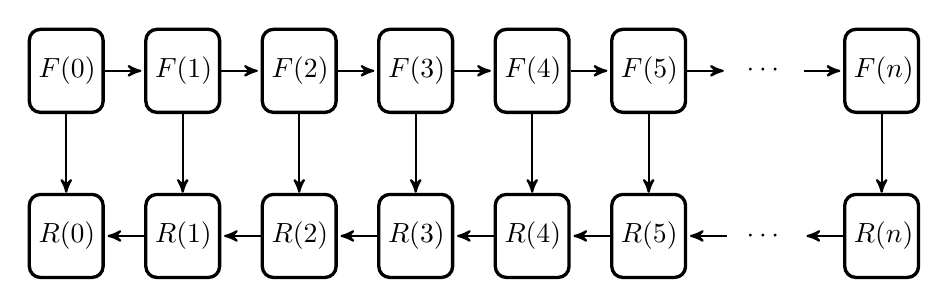
\begin{tikzpicture}
  [node distance=.5cm,
  start chain=1 going right,start chain=2 going left]
     \node[punktchain, join, on chain=1] (t1) {$F(0)$};
     \node[punktchain, join, on chain=1] (t2)      {$F(1)$};
     \node[punktchain, join, on chain=1] (t3)      {$F(2)$};
     \node[punktchain, join, on chain=1] (t4) {$F(3)$};
     \node[punktchain, join, on chain=1] (t5) {$F(4)$};
     \node[punktchain, join, on chain=1] (t6) {$F(5)$};
     \node[punktchain, join, draw=none, on chain=1] (ellipsis1) {$\cdots$};
     \node[punktchain, join, on chain=1] (tn) {$F(n)$};

\node[punktchain, below=1cm of tn, on chain=2] (atn) {$R(n)$};
\node[punktchain, join, draw=none, on chain=2] (ellipsis2) {$\cdots$};
     \node[punktchain, join, on chain=2] (at6)      {$R(5)$};
     \node[punktchain, join, on chain=2] (at5)      {$R(4)$};
     \node[punktchain, join, on chain=2] (at4) {$R(3)$};
     \node[punktchain, join, on chain=2] (at3) {$R(2)$};
     \node[punktchain, join, on chain=2] (at2) {$R(1)$};
     \node[punktchain, join, on chain=2] (at1) {$R(0)$};

\draw[|-,-|,->, thick,] (t1.south) |-+(0,-1em)-| (at1.north);
\draw[|-,-|,->, thick,] (t2.south) |-+(0,-1em)-| (at2.north);
\draw[|-,-|,->, thick,] (t3.south) |-+(0,-1em)-| (at3.north);
\draw[|-,-|,->, thick,] (t4.south) |-+(0,-1em)-| (at4.north);
\draw[|-,-|,->, thick,] (t5.south) |-+(0,-1em)-| (at5.north);
\draw[|-,-|,->, thick,] (t6.south) |-+(0,-1em)-| (at6.north);
\draw[|-,-|,->, thick,] (tn.south) |-+(0,-1em)-| (atn.north);
  \end{tikzpicture}
\end{center}
\caption{The dataflow pattern that is typical of adjoint-based optimization problems}
\label{fig:dataflow}
\end{figure}


Data compression is also increasingly used to reduce the memory footprint of
scientific applications. General purpose data compression algorithms like Zlib
(which is a part of gzip)~\cite{deutsch1996zlib}, and compression algorithms for
video and image data such as JPEG-2000~\cite{skodras2001jpeg} have been
presented in previous work. More recently, special purpose compression
algorithms for floating-point scientific data have been developed, such as ZFP
or SZ~\cite{Kaklamanis:2012aa,lindstrom2014fixed,di2018efficient}.

Lossless algorithms guarantee that the exact original data can be recovered
during decompression, whereas lossy algorithms introduce an error, but often
guarantee that the error does not exceed certain absolute or relative error
metrics. Typically, lossy compression is more effective in reducing the data
size. Most popular compression packages offer various settings that allow a
tradeoff between compression ratio, accuracy, and compression and decompression
time. In this work we use the ZFP package to perform lossy compression.

It is worth noting that another data reduction strategy is to typecast values
into a lower precision format, for example, from double precision to single
precision. This can be seen as a computationally cheap lossy compression
algorithm with a compression ratio of $2$.

Perhaps counterintuitively, compression can not only reduce the memory
footprint, but also speed up an application. Previous work has observed that the
compression and decompression time can be less than the time saved from the
reduction in data that needs to be communicated across MPI nodes or between a
GPU and a host computer~\cite{gpu-compression}.

Another way of using compression to speed up adjoint-based methods is to use it \emph{instead} of
checkpointing. If the compression ratio is sufficient to fit the
entire data in memory, checkpointing is no longer necessary. Previous
work has discussed this in the context of computational
fluid dynamics~\cite{cyr2015towards} and seismic inversion using
compression algorithms specifically designed for
wavefields~\cite{dalmau2014lossy,boehm2016wavefield}.

In this paper, we extend the previous studies by \emph{combining} checkpointing
and compression. This is obviously useful when the data does not fit in the
available memory even after compression, for example for very large adjoint
problems, or for problems where the required accuracy limits the achievable
compression ratios.

Compared to the use of only checkpointing without compression, our
combined method often improves performance. This is a consequence of
the reduced size of stored program states, allowing more program
states to be stored during the forward computation. This in turn
reduces the amount of recomputation that needs to be performed. On the
other hand, the compression and decompression itself takes time. We
therefore provide a comprehensive performance model that predicts
whether the combined method is beneficial, that is, whether the time
spent compressing and decompressing is less than the time saved by
reduced recomputations.

For benchmarking we used a dual-socket
Intel(R) Xeon(R) Platinum 8180M @ 2.50 Ghz (28 cores each), henceforth
called Skylake. We discuss performance results for varying error tolerances for
the lossy ZFP compression algorithm ranging from $10^0$ to $10^{-15}$, and different
types of forward and adjoint computations that vary in their ratio between
compute cost and state size. 

Our aim is to make this discussion independent of the hardware, application and
compression algorithm. We therefore do not discuss whether or not the accuracy
of the decompressed data is sufficient for our application, or whether
other algorithms might achieve a better accuracy/compression tradeoff.

\section{Test case using Devito and pyRevolve}
We use Devito~\cite{devito-api,devito-compiler} to solve forward and adjoint
wave equation problems. Devito is a domain-specific language that enables the
rapid development of finite-difference solvers from a high-level description
of partial differential equations. The simplest version of the seismic wave
equation is the acoustic isotropic wave equation defined as:
\begin{equation}
m(x)\frac{\partial^2 u(t, x)}{\partial t^2} - \Laplace u(t, x) = q(t, x),
\label{eqn:wave}
\end{equation}
where $m(x) = \frac{1}{c^2(x)}$ is the squared slowness, $c(x)$ the spatially
dependent speed of sound, $u(t, x)$ is the pressure wavefield, $\Laplace u(t, x)$ denotes the laplacian of the wavefield and $q(t, x)$ is a source term.
Some of our experiments in Section \ref{sec:results} are performed using a more accurate
and more complex version of this equation called Tilted Transverse Isotropy
(TTI)~\cite{zhang2011stable} that takes into account the anisotopic propagation of waves in the earth subsurface (directional dependency of the speed of sound). We leave the TTI equations out of this paper
for brevity. 

The solution to equation~\ref{eqn:wave} forms the forward problem. The seismic inversion problem minimizes the misfit between simulated and observed signal given by:
\begin{equation}
\min_{m} \phi_s(m) = \frac{1}{2} \left\lVert d_{sim} - d_{obs} \right\rVert_2^2.
\end{equation}

This optimization problem is usually solved using gradient based methods such as steepest descent,
where the gradient is computed using the adjoint-state method that involves
the data-flow pattern from figure \ref{fig:dataflow}.

The values of $m(x)$ used in this work are derived from the Overthrust
model~\cite{aminzadeh1996three} over a grid of $287 \times 881 \times 881$
points, including an absorbing layer of 40 points on each side. The grid spacing
is $25m$ in space. The propagation time is $4sec$ that corresponds to 2500 timesteps. The wave field
at the final time is shown in Figure~\ref{fig:uncompressed}, and only this field
was used for the compression experiments in this paper. The uncompressed size of
this single time step field is just under 900MB.

\begin{figure}
\begin{center}
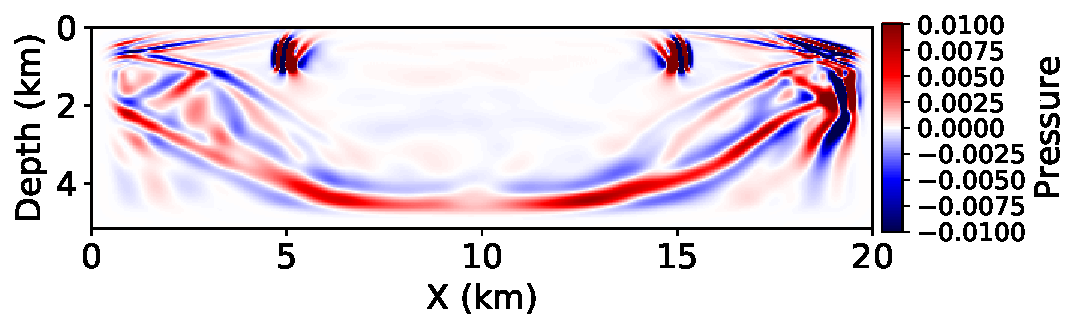
\includegraphics[width=0.8\linewidth]{images/uncompressed.pdf}
\end{center}
\caption{Cross-section of the wavefield used as a reference sample for
  compression and decompression. This field was formed after a Ricker
  wavelet source was placed at the surface of the model and the wave propagated for 2500
  timesteps. This is a vertical (x-z) cross-section of a 3D field, taken at
  the $y$ source location}
\label{fig:uncompressed}
\end{figure}

To implement Revolve with Devito, we use pyRevolve~\cite{kukreja2018high} which
is a python wrapper for the Revolve algorithm. The performance model in
section~\ref{sec:performance_model} assumes that the implementation is similar
to pyRevolve, which stores a checkpoint by copying a portion of the operator's
working memory to the checkpointing memory and similarly loads a checkpoint by
copying from the checkpointing memory to the operator's working memory. Although
a perfect implementation of checkpointing may be able to avoid these copies, the
overhead attached to these copies can be ignored for an operator that is
sufficiently computationally intensive. However, we include the overheads in the
model to verify this assumption. 

\section{Compression algorithms}
\subsection{Lossless}
We use the python package \emph{blosc}~\cite{blosc}, which includes implementations for
six different lossless compression algorithms, namely ZLIB, ZSTD, BLOSCLZ,
LZ4, LZ4HC and Snappy. An exhaustive search over all available parameters 
resulted in a maximum compression ratio of 1.18x. We therefore focus on lossy
compression in the remainder of this work.

\subsection{Lossy}
We use the lossy compression package ZFP~\cite{lindstrom2014fixed} developed in
C. To use ZFP from python, we developed a python wrapper for the reference
implementation of ZFP.

\begin{figure}
\begin{center}
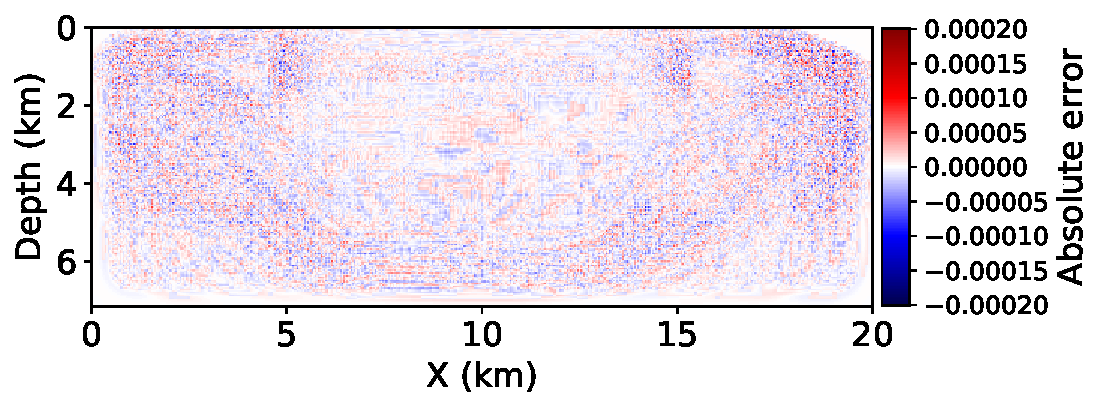
\includegraphics[width=0.8\linewidth]{images/errors.pdf}
\end{center}
\caption{Cross-section of the field that shows errors introduced
  during compression and decompression using the fixed-tolerance
  mode. It is interesting to note that the errors are more or less
  evenly distributed across the domain with only slight variations
  corresponding to the wave amplitude (from the field plot in figure
  \ref{fig:uncompressed}. A small block-like structure characteristic of
  ZFP can be seen.}
\label{fig:decompressed_error}
\end{figure}

ZFP supports three compression modes, namely fixed-tolerance, fixed-precision
and fixed-rate. The fixed-tolerance mode limits the absolute error, while the
fixed-precision mode limits the relative error to some user-specified value.
The fixed-rate mode achieves a guaranteed compression ratio requested by the
user, but does not provide any bounds on accuracy loss.
Figure~\ref{fig:tolerance_cf_plot} shows compression ratios for a variety of
settings for the three modes.

The compression ratio achieved per unit time spent during compressing
and decompressing was seen to be highest in the fixed-tolerance mode
albeit with highly unpredictable compression ratios. Figure
\ref{fig:decompressed_error} shows the spatial distribution of the
error after compression and decompression, compared to the original
field, using fixed-tolerance mode.

In our experiments using Devito, the time required to compress a checkpoint was
in the same order of magnitude as the time taken to compute a timestep.

\begin{figure}
\begin{center}
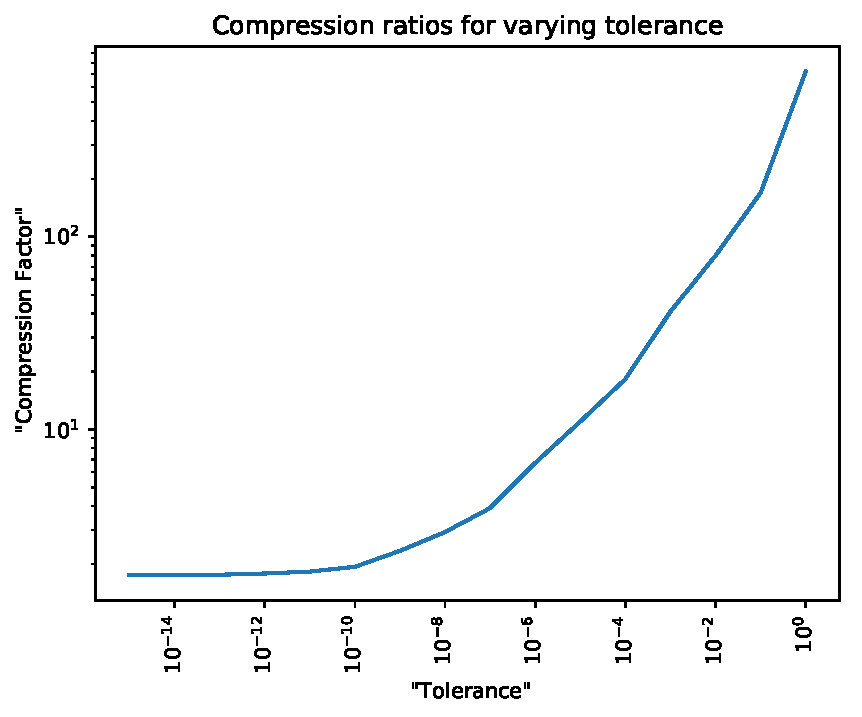
\includegraphics[width=0.9\linewidth]{images/tolerance-cf-richter.pdf}
\end{center}
\caption{Compression ratios achieved on compressing the wavefield. We
  define compression ratio as the ratio between the size of the
  uncompressed data and the compressed data. The dashed line
  represents no compression. The highlighted point corresponds to the
  setting used for the other results here unless otherwise specified.}
\label{fig:tolerance_cf_plot}
\end{figure}

\section{Performance model for a combination of Revolve and compression}
\label{sec:performance_model}
We assume that the computation of a single forward time step takes the same wall
time as the computation of a single reverse time step. We denote this time as
$\mathbf{C}$. For a simulation with $\mathbf{N}$ timesteps, the minimum wall time required
for the full forward-adjoint evaluation is given by
\begin{equation}
T_N = 2 \cdot \mathbf{C} \cdot \mathbf{N}.
\end{equation}
If the size of a single timestep in memory is given by $\mathbf{S}$, this
requires a memory of at least size $\mathbf{S} \cdot \mathbf{N}$. If sufficient memory
is available, no checkpointing or compression is needed.

If the memory is smaller than $\mathbf{S} \cdot \mathbf{N}$, Revolve provides
a strategy to solve for the adjoint field by storing a subset of the $\mathbf{N}$ total checkpoints
and recomputing the remaining ones. The overhead introduced by this method can be broken down into
the recomputation overhead $\mathbf{O}_R$ and the storage overhead $\mathbf{O}_S$. The recomputation
overhead is the amount of time spent in recomputation, given by
\begin{equation}
\mathbf{O}_R(N, M) = p(N, M) \cdot \mathbf{C},
\end{equation}
where $p(N, M)$ is the minimum number of recomputed steps from \cite{griewank2000algorithm}, reproduced
here in equation \ref{eqn:recompute}.
\begin{figure*}
\begin{equation}
p(N, M) = \begin{cases}
      N(N-1) /2, & \text{if}\ M=1 \\
      \min\limits_{1<=\widetilde{N}<=N} \{\widetilde{N} + \mathbf{O}_R(\widetilde{N}, M) + \mathbf{O}_R(N-\widetilde{N}, M-1)\}, & \text{if}\ M>1
    \end{cases}
    \label{eqn:recompute}
\end{equation}
\end{figure*}
In equation \ref{eqn:recompute}, M is the number of checkpoints that can be
stored in memory. Note that for $M >=N$, $\mathbf{O}_R$ would be zero. For $M <
N$, $\mathbf{O}_R$ grows rapidly as M is reduced relative to N. 

In an ideal implementation, the storage overhead $\mathbf{O}_S$ might be zero, since the computation could
be done ``in-place'', but in practice, checkpoints are generally stored in a separate section of memory and they
need to be transferred to a ``computational'' section of the memory where the compute is performed, and then
the results copied back to the checkpointing memory. This copying is a common feature of checkpointing
implementations, and might pose a non-trivial overhead in scenarios where the computation is heavily bandwidth-bound. 
This storage overhead is given by
\begin{equation}
\mathbf{O}_{SR} = \mathbf{N}_W \cdot \frac{\mathbf{S}}{\mathbf{B}} +
\mathbf{N}_R \cdot \frac{\mathbf{S}}{\mathbf{B}}.
\label{eqn:storage}
\end{equation}
where $\mathbf{N}_W$ is the total number of times Revolve writes
checkpoints for a single run, $ \mathbf{N}_R$ is the number of times
checkpoints are read, and $\mathbf{B}$ is the memory bandwidth of the
target system. The total time to solution becomes
\begin{equation}
T_R = 2 \cdot \mathbf{C} \cdot \mathbf{N} + \mathbf{O}_R(N, M) + \mathbf{O}_S.
\end{equation} 
By using compression, the size of each checkpoint is reduced and therefore the
number of checkpoints available is increased ($M$ in equation
\ref{eqn:recompute}). This reduces the recomputation overhead $\mathbf{O}_R$,
while at the same time adding overheads related to compression and decompression
in $\mathbf{O}_S$.
To be beneficial, the reduction in $\mathbf{O}_R$ must offset the increase in 
$\mathbf{O}_S$, leading to an overall decrease in the time to solution $T$.

Our performance model assumes
 that the compression algorithm behaves uniformly
across the different time steps of the simulation, i.e. that we get the same compression ratio, compression time and 
decompression time, no matter which of the $N$ possible checkpoints we try to compress/decompress. The storage overhead
now becomes
\begin{equation}
\mathbf{O}_{SR} = \mathbf{N}_W \cdot \left(\frac{\mathbf{S}}{\mathbf{F}
  \cdot \mathbf{B}} + t_c\right) + \mathbf{N}_R \cdot
\left(\frac{\mathbf{S}}{\mathbf{F} \cdot \mathbf{B}} + t_d\right)
\end{equation}
where $\mathbf{F}$ is the compression ratio (i.e. the ratio between the uncompressed and compressed checkpoint), and $t_c$
and $t_d$ are compression and decompression times, respectively. At the same
time, the recomputation overhead decreases
because $\mathbf{F}$ times more checkpoints are now available.

\section{Results}
\label{sec:results}
We can distinguish three different scenarios, depending on the amount of
available memory.
\begin{enumerate}
\item If the memory is insufficient even with compression to store the entire
trajectory, one can either use checkpointing only, or combine checkpointing with
compression.
\item If the available memory is not sufficient to store the uncompressed
trajectory, but large enough to store the entire compressed trajectory, we study
the two possible strategies: Either use compression only, or use checkpointing
only.
\item If the available system memory is large enough to hold the entire
uncompressed trajectory, neither compression nor checkpointing is necessary.
\end{enumerate}
All three scenarios can be seen in figure~\ref{fig:varying_memory}.
The second scenario was studied in previous work~\cite{cyr2015towards}, while
the combined method is also applicable to the first scenario, for which previous
work has only used checkpointing without compression.

We can identify a number of factors that make compression more likely to be
beneficial compared to pure checkpointing: A very small system memory size and a
large number of time steps lead to a rapidly increasing recompute factor, and
compression can substantially reduce this recompute factor. This can be seen in
figures~\ref{fig:varying_memory} and~\ref{fig:varying_nt}.

The extent to which the recompute factor affects the overall runtime also
depends on the cost to compute each individual time step. If the compute cost
per time step is large compared to the compression and decompression cost, then
compression is also likely to be beneficial, as shown in
figure~\ref{fig:varying_compute}. As the time per time step increases and the
compression cost becomes negligible, we observe that the ratio between the runtime
of the combined method and that of pure checkpointing is only determined by the
difference in recompute factors.

\begin{figure}
\begin{center}
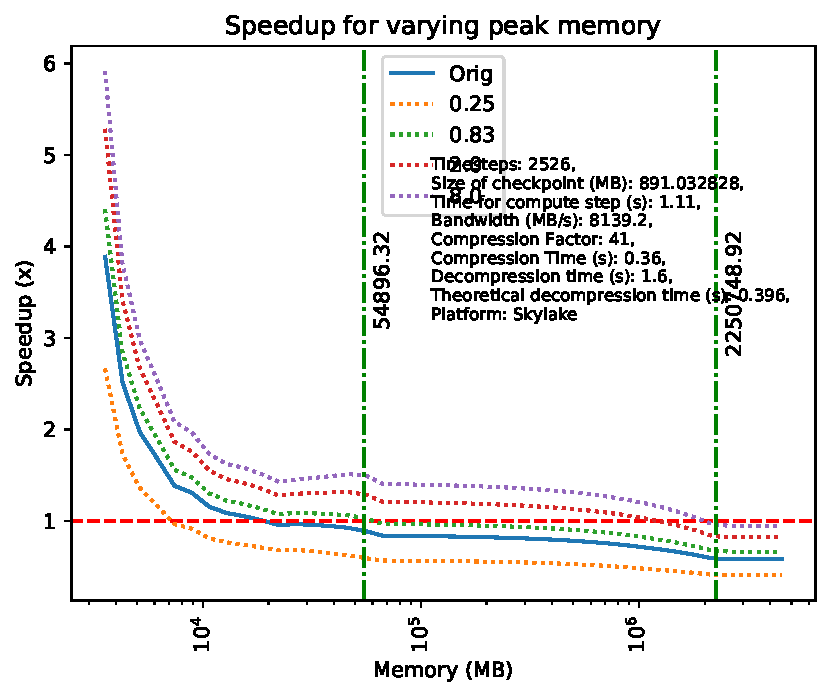
\includegraphics[width=0.9\linewidth]{images/varying-memory.pdf}
\end{center}
\caption{The speedups predicted by the performance model for varying
  memory. The baseline
(1.0) is the performance of a Revolve-only implementation under the
same conditions. The different curves represent kernels with differing
compute times (represented here as a factor of the sum of compression
and decompression times). The first vertical line at $~$ 53GB marks the
spot where the compressed wavefield can completely fit in memory and
Revolve is unnecessary if using compression. The second vertical line
at $~$ 2.2 TB marks the spot where the entire uncompressed wavefield can
fit in memory and neither Revolve nor compression is necessary. The
region to the right is where these optimisations are not necessary or
relevant. The middle region has been the subject of past studies using
compression in adjoint problems. The region to the left is the focus
of this paper.}
\label{fig:varying_memory}
\end{figure}

\begin{figure}
\begin{center}
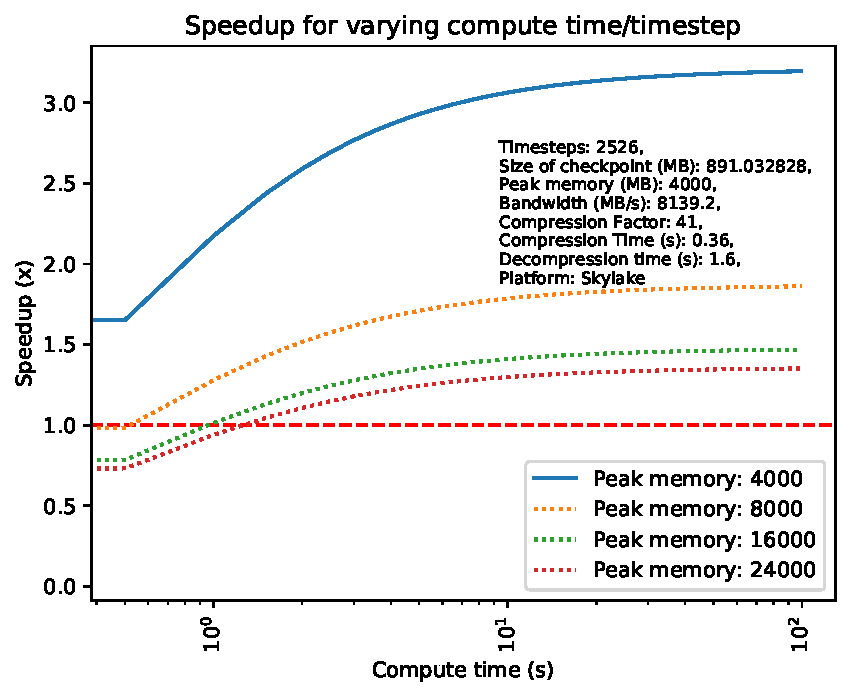
\includegraphics[width=0.9\linewidth]{images/varying-compute.pdf}
\end{center}
\caption{The speedups predicted by the performance model for varying
  compute cost. The baseline
(1.0) is the performance of a Revolve-only implementation under the
same conditions. The benefits of compression drop rapidly if the
computational cost of the kernel that generated the data is much lower
than the cost of compressing the data. For increasing computational
costs, the benefits are bounded.}
\label{fig:varying_compute}
\end{figure}

\begin{figure}
\begin{center}
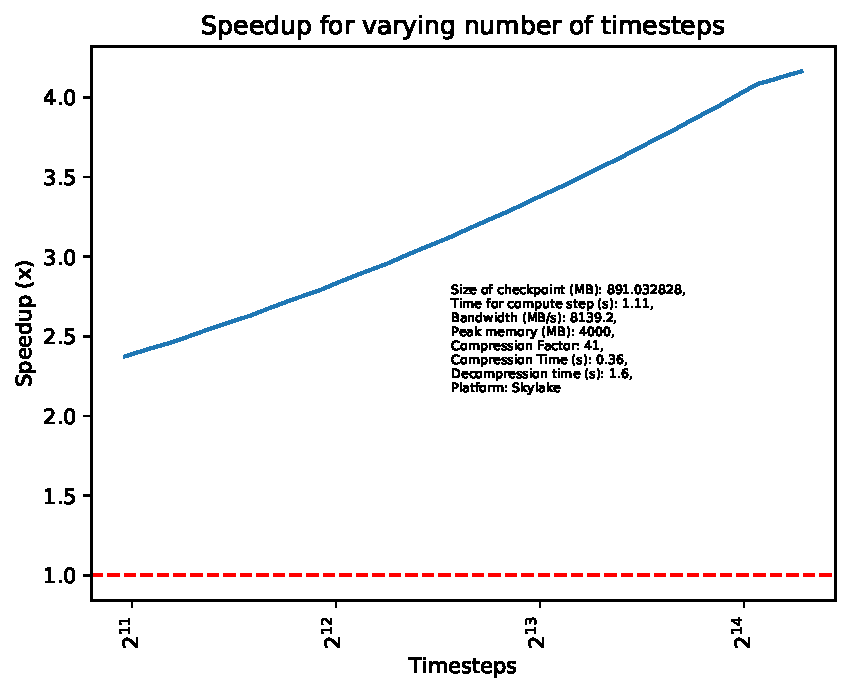
\includegraphics[width=0.9\linewidth]{images/varying-nt.pdf}
\end{center}
\caption{The speedups predicted by the performance model for varying
  number of timesteps to be reversed. The baseline
(1.0) is the performance of a Revolve-only implementation under the
same conditions. It can be seen that compression becomes more
beneficial as the number of timesteps is increased.}
\label{fig:varying_nt}
\end{figure}

\section{Conclusions and Future work}
We use lossy compression to reduce the computational overhead of
checkpointing in an adjoint computation used in full waveform
inversion, a common method in seismic imaging applications whose
memory footprint commonly exceeds the available memory size in high
performance computing systems. We also developed a performance model
that computes whether or not the combination of compression and
checkpointing will outperform pure checkpointing or pure compression
in a variety of scenarios, depending on the available memory size,
computational intensity of the application, and compression ratio and
throughput of the compression algorithm. Our current result has
several limitations that we plan to address in future work:
\begin{itemize}
\item We do not discuss the accuracy of the results after decompression. This
depends on the application, compression algorithm, and affects the achievable
compression ratios. Our performance model only requires knowledge of the
compression time and ratio, and it is up to the user of this model to determine
what accuracy is needed and thus what compression ratio is realistic for their
application.
\item We only present results using the ZFP compression library. It
would be interesting to try a greater variety of compression
algorithms.
\item ZFP only supports serial decompression. If ZFP supported
parallel decompression, our experiments would likely show a geater region in
which the combined method is faster than pure checkpointing. Furthermore, ZFP
only supports fields with up to three dimensions, while
exploiting similarities between fields at different time steps may yield a
better compression ratio.
\item Our performance model is based on uniform compression ratios and
times.  However, many applications, including FWI, are likely to have
initial conditions that contain little information and are easily
compressed, and the compression ratio gradually declines as the field
becomes more complex. We based our experiments on the final wave
field, which is presumably difficult to compress.
\item In comparing pure compression with pure checkpointing, we assume
that every checkpoint is compressed and decompressed. However, if the
available memory is only slightly less than the required memory, an
implementation that compresses only a subset of the checkpoints might
outperform the expectations of our model.
\item We do not discuss multi-level checkpointing, where some
checkpoints are stored on a slower, larger device. We expect
compression to be beneficial in these scenarios due to reduced data
transfer sizes.
\end{itemize}

\section*{Acknowledgment}
This work was funded by the Intel Parallel Computing Centre at
Imperial College London and EPSRC EP/R029423/1. 
This work was supported by the U.S. Department of Energy, Office of Science,
Office of Advanced Scientific Computing Research, Applied Mathematics and
Computer Science programs under contract number DE-AC02-06CH11357.
We would also like to acknowledge the support from the SINBAD II project and
the member organizations of the SINBAD Consortium.

We gratefully acknowledge the computing resources provided and operated by the
Joint Laboratory for System Evaluation (JLSE) at Argonne National Laboratory.


\bibliographystyle{plain}
\bibliography{compression}

\vfill
\begin{flushright}
\normalsize
\framebox{\parbox{3in}{The submitted manuscript has been created by UChicago
Argonne, LLC, Operator of Argonne National Laboratory (`Argonne'). Argonne, a
U.S. Department of Energy Office of Science laboratory, is operated under
Contract No. DE-AC02-06CH11357. The U.S. Government retains for itself, and
others acting on its behalf, a paid-up nonexclusive, irrevocable worldwide
license in said article to reproduce, prepare derivative works, distribute
copies to the public, and perform publicly and display publicly, by or on behalf
of the Government.  The Department of Energy will provide public access to these
results of federally sponsored research in accordance with the DOE Public Access
Plan.\newline \url{http://energy.gov/downloads/doe-public-access-plan}.}}
\end{flushright}

\end{document}
